% Nexus robot description

\chapter{Nexus Robot}
\label{ch:nexus}

This chapter will talk about the Nexus Robot, a small 2--wheeled robot that was used as a testbed for different SLAM algorithms, before applying them on the PEV.

Another purpose for this robot is to serve as an educational platform, by creating interfaces for students of different segments to learn about mobile robots and Autonomous Vehicles.

The last reason to research on these smaller robots is to explore the idea of using them as a 'last meter' delivery system, making intra--office communication much faster and bridging the gap between a platform like the PEV and the end user/client.

\section{Description of the robot}

The \href{https://www.nexusrobot.com/}{Nexus Robot} is a 2 wheeled differential drive platform as shown in \autoref{fig:nexus}, that is used for educational robotics and costs around 500\$.
\begin{figure}[htb]
  \centering
  \subfloat[Nexus robot as sold]{\frame{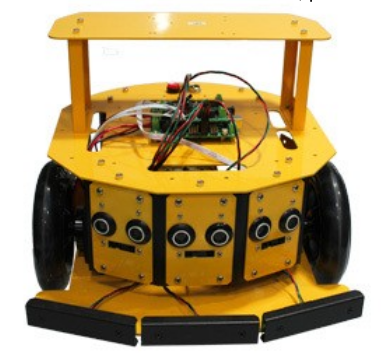
\includegraphics[width=.45\linewidth]{pictures/04/nexus}}} \quad
  \subfloat[Setup]{\frame{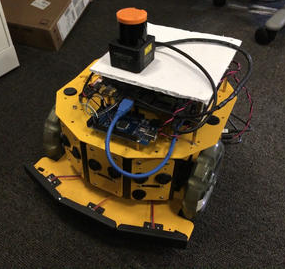
\includegraphics[width=.45\linewidth]{pictures/04/nexusetup1}}}
  \caption{Nexus robot}
  \label{fig:nexus}
\end{figure} 

The body of the robot is made of aluminum and its dimensions are 30cm in circumference and 20cm in height. Due to its size it is ideal for indoor navigation and the fact that is a differential drive improves its manouverability in those environments. 

Generally, it does not come with very advanced sensors, thus in order to perform autonomous navigation tasks its capabilities had to be enhanced with more sensors and computing units. Those will be described in the following sections.

\subsection{Hardware}

\parunder{Sensors}The sensors that come with and were added to the platform are:
\begin{itemize}
  \item \textbf{Sonar}: The robot comes with 3 low--range ultrasonic sensors that are originally intended for obstacle detection. However, they were not used in this experiments.

  \item \textbf{Bumper sensors}: It also comes with 3 bumber sensors to detect collisions but those have not been used either.

  \item \textbf{Wheel encoders}: Each wheel comes with a 2--channel encoder (A and B) to calculate the linear and rotational speeds.

  \item \textbf{Lidars}: 2 diiferent lidars were used throught the experiments (\autoref{fig:lidars}):
  \begin{itemize}
    \item \href{https://www.slamtec.com/en/Lidar/A2}{RPLidar A2}: It is an 12m range lidar, with a 360\textsuperscript{o} field of view and outputs 4000 points per/second (400 per revolution). The connection is done via USB adapter. 

    \item \href{https://www.hokuyo-usa.com/products/scanning-laser-rangefinders/ust-10lx}{Hokuyo UST-10LX}: The range of this lidar is of 10m, with a 270\textsuperscript{o} field of view and more than 40.000 points per second (1080 per scan). This laser uses ethernet to connect to the computer.
  \end{itemize}

  \begin{figure}[htb]
    \centering
    \subfloat[RPLidar A2]{\frame{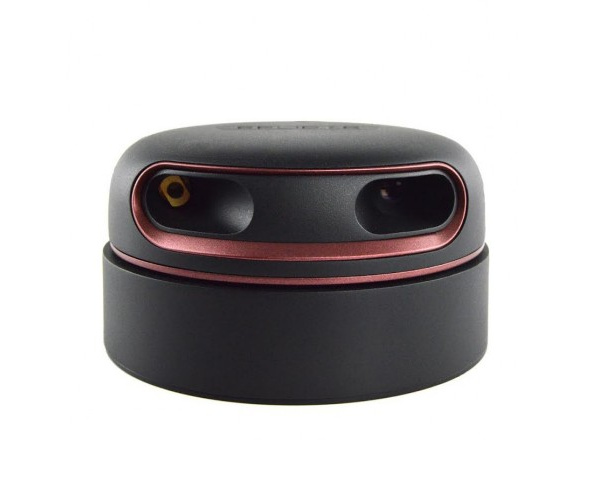
\includegraphics[width=.45\linewidth]{pictures/04/rplidar}}} \quad
    \subfloat[Hokuyo UST-10LX]{\frame{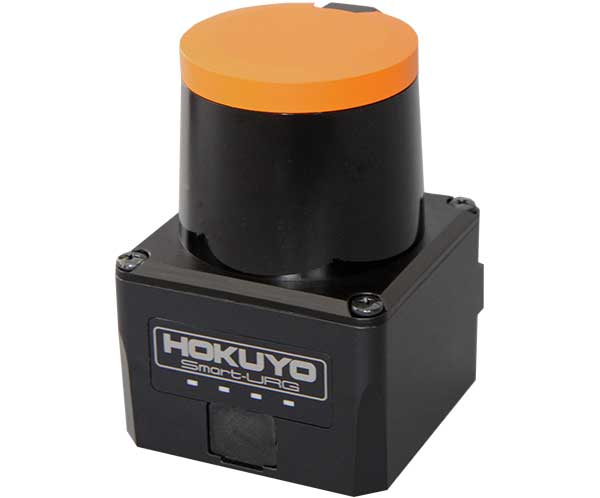
\includegraphics[width=.45\linewidth]{pictures/04/hokuyo}}}
    \caption{Lidars used in the Nexus robot}
    \label{fig:lidars}
  \end{figure} 
\end{itemize}  

\parunder{Actuators} The robot comes with 2 12V DC motors, one for each wheel and each one has 2 control pins: one for rotation direction and one for speed.

\parunder{Control} Control comes from 2 platforms:
\begin{itemize}
  \item Controller board: Connected to a 12V power supply, it is in charge of sending power and control commands to the DC motors. It is equipped with an ATMega 168 and can be programmed with the Arduino IDE, but the low amount of memory (16KB) makes the controller's behavior unstable when bridged to ROS.

  \item \href{https://store.arduino.cc/usa/arduino-mega-2560-rev3}{Arduino Mega}: It is one of the most complex \href{https://store.arduino.cc/usa/}{Arduino} boards (\autoref{fig:mega}), with 54 digital pins, 16 analog pins and a memory of 256KB. That capacity is important since the board was bridged to communicate with the ROS system, and ROS libraries occupy a notable amount of space on microcontrollers.
\end{itemize}

\begin{figure}[htb]
  \centering
  \frame{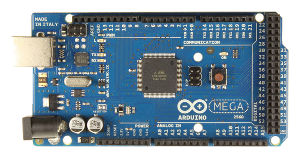
\includegraphics[width=.8\linewidth]{pictures/04/mega}}
  \caption{Arduino Mega board layout}
  \label{fig:mega}
\end{figure}

\parunder{Computing} The computations onboard are performed by a \href{https://www.nvidia.com/en-us/autonomous-machines/embedded-systems-dev-kits-modules/}{Jetson TX2 Developer platform} developed by Nvidia (\autoref{fig:tx2}). This device is part of a branch of development computers aimed at tasks like autonomous navigation or deep learning. Some of the features are: 32GB hard--drive, 8GB of RAM and a 256--core GPU.

\begin{figure}[htb]
  \centering
  \frame{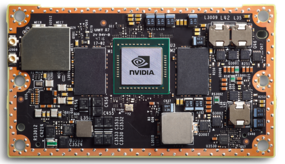
\includegraphics[width=.8\linewidth]{pictures/04/tx2}}
  \caption{Jetson TX2 module}
  \label{fig:tx2}
\end{figure}

The Operating System is Ubuntu 16.04 and it has libraries such as CUDA, CUDNN, OpenCV and TensorRT preinstalled in order to perform all sorts of deep learning and artificial intelligence tasks that require parallel computing. It is also compatible with ROS, thus making the TX2 an interesting device for self--driving vehicles.

\section{Setup}
The conceptual setup of the Nexus robot is depicted in \autoref{fig:nexussch}.
\begin{figure}[htb]
  \centering
  \frame{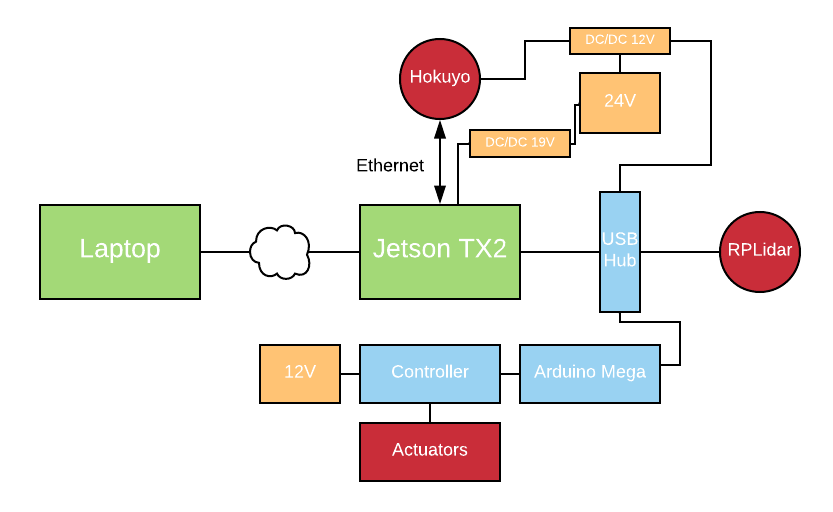
\includegraphics[width=\linewidth]{pictures/04/nexussch}}
  \caption{Nexus setup conceptual overview}
  \label{fig:nexussch}
\end{figure}  

As it can be seen, the Jetson TX2 is in charge of running all the sensors and controllers and then it is connected via WiFi to the laptop. The latter stores the data from the experiments and visualizes it on RVIZ. This connection is possible thanks to the networking capabilities of ROS.

\subsection{Control}

It was briefly mentioned above how the Arduino controlled the actuators of the robot. In this subsection this explanation will be expanded.

Both motors are set to Pulse--Width Modulation (PWM) mode and each one has 2 pins to be set, as shown in \autoref{tab:nexuscontrol}. \
\begin{table}[htb]
  \centering
  \begin{tabular}{lll}
  \hline
  \textbf{Pin} & \textbf{Name} & \textbf{Description} \\ \hline
  4 & M1 & Direction control of Motor 1 \\ \hline
  5 & E1 & PWM control of Motor 1 \\ \hline
  6 & E2 & PWM control of Motor 2 \\ \hline
  7 & M2 & Direction control of Motor 2 \\ \hline
  \end{tabular}
  \caption{Pin controls of the motors}
  \label{tab:nexuscontrol}
\end{table}

Motors 1 and 2 correspond to the left and right wheels. As for the encoders, each one has 12 pulses per revolution, 2 channels and a gearbox ratio of 64:1. That yields $64\cdot 12\cdot 4 = 3072$ pulses per revolution. In order to obtain a pulse every time there is a change, 2 interrupts have to be attached to each encoder, one for channel. From the Arduino IDE this can be done as  in \autoref{lst:interrupt}, where ELA and ELB are the pins connected to channel A and B of the left encoder.
\begin{lstlisting}[float=htb,language=C,frame=htb,caption={Attaching interrupts},label=lst:interrupt] 
  attachInterrupt(digitalPinToInterrupt(ELA), doEncoderlA, CHANGE);
  attachInterrupt(digitalPinToInterrupt(ELB), doEncoderlB, CHANGE);
\end{lstlisting}

In \autoref{fig:controlsetup}, a schematic of the wiring of the system is shown.
\begin{figure}[htb]
  \centering
  \frame{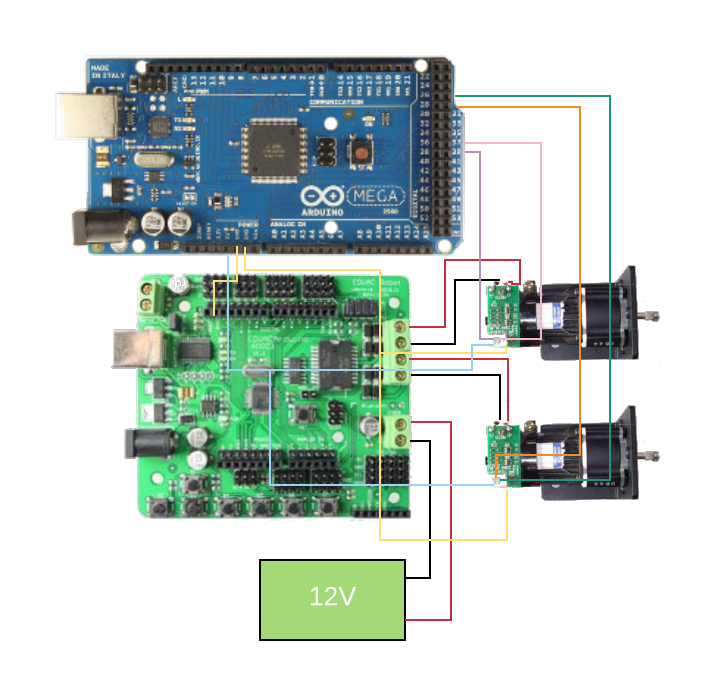
\includegraphics[width=.85\linewidth]{pictures/04/control}}
  \caption{Nexus robot control wiring}
  \label{fig:controlsetup}
\end{figure}  

\subsection{Speed commands}
Speed commands come in the form of the ROS message type \texttt{Twist.h} and then are translated to left and right wheel speed. 2 different sources output speed commands:
\begin{itemize}
  \item \textbf{Joystick}: When recording data to map the environment a \href{https://www.logitechg.com/en-us/products/gamepads/f710-wireless-gamepad.html}{Logitech gamepad} was used to control the robot.

  \item \textbf{Navigation system}: When running in autonomous mode, speed commands come from the navigation stack, specifically the local planner. 
\end{itemize}  

\subsection{ROS package}
All the functionalities of the Nexus Robot have been gathered in a collection of ROS packages that can be found on \href{https://github.com/yagoliz/nexus_robot_autonomous_navigation}{Github}. \autoref{tab:nexusros} is offered as an explanation of the different modules provided:
\begin{table}[h]
  \centering
  \begin{tabular}{lp{7cm}}
  \hline
  \textbf{Package name} & \textbf{Description} \\ \hline
  minion\_teleop & Scripts to run the joystick and send speed commands to the robot \\ \hline
  nexus\_robot\_2wd & Contains the Arduino code, hardware rules and odometry nodes \\ \hline
  nexus\_robot\_cartographer & Scripts to run Google's cartographer on the nexus robot \\ \hline
  nexus\_robot\_localization & Contains the autonomous navigation software (localization, path planning and move\_base) \\ \hline
  nexus\_robot\_mapping & Scripts to run Gmapping or Hector SLAM \\ \hline
  nexus\_robot\_msgs & Custom ROS messages for the platform \\ \hline
  \end{tabular}
  \caption{ROS packages to control the nexus robot}
  \label{tab:nexusros}
  \end{table}

\section{Indoor SLAM with Nexus}

Once the main aspects of the Nexus robot setup have been described, this section will show the results of the SLAM performed in 3 different scenerarios: \textbf{City Science group's lunch room}, \textbf{City Science group} and the \textbf{Media Lab's third floor}.

The algorithms employed with the Nexus robot have been \textbf{Gmapping} and \textbf{Hector SLAM}. For every environment Gmapping will be shown first and then Hector.

\subsection{Autonomous navigation workflow}
For every environment the procedure to perform SLAM and subsequent navigation was the same: 4 test runs are performed, and basic sensor data is recorded into bag files: encoder tics and laser data.  

2 of those recorded files were used to perform SLAM and a considerable amount of maps was obtained. The best map of the batch was then used to test localization and path planning algorithms. Once the results from tests were correct, online runs were carried.

\subsection{Lunch Room}

The lunch room is a small (5$\times$5 m\textsuperscript{2}) space where the City Science has its meetings. It is an ideal place to start with mapping algorithms and measure their robustness to different parameters.

\parunder{Gmapping in Lunch Room} The tests performed with gmapping are shown in \autoref{tab:gmappinglunch}:
\begin{table}[h]
  \centering
  \begin{tabular}{lc}
  \hline
  \textbf{Parameter} & \textbf{Range} \\ \hline
  Default & - \\ \hline
  Linear update rate & {[}0.1-1.0{]} \\ \hline
  Angular update rate & {[}0.1-1.0{]} \\ \hline
  Number of iterations for the scanmatcher & {[}0-10{]} \\ \hline
  Number of particles in the filter & {[}1-30{]} \\ \hline
  \end{tabular}
  \caption{Tests with Gmapping in the lunch room}
  \label{tab:gmappinglunch}
\end{table}

\autoref{fig:gmappinglunchdef} shows the occupancy grid map with the default values. The result is satisfactory and it would suffice to peform navigation. However, in order to test the robustness of the algorithm, the rest of the cases are shown.
\begin{figure}[h]
  \centering
  \frame{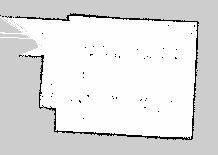
\includegraphics[width=.9\linewidth]{pictures/04/lunch_room/gmapping/linearup100}}
  \caption{Lunch room map with defaults for Gmapping}
  \label{fig:gmappinglunchdef}
\end{figure}  

\begin{figure}[t!]
  \centering
  \subfloat[Linear update every 0.1 m]{\frame{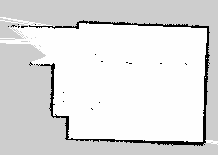
\includegraphics[width=.45\linewidth]{pictures/04/lunch_room/gmapping/linearup010}}} \quad
  \subfloat[Linear update every 1.0 m]{\frame{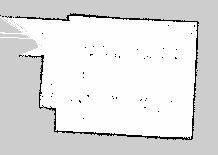
\includegraphics[width=.45\linewidth]{pictures/04/lunch_room/gmapping/linearup100}}} \\
  \subfloat[Angular update every 0.1 rad]{\frame{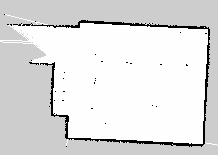
\includegraphics[width=.45\linewidth]{pictures/04/lunch_room/gmapping/angularup010}}} \quad
  \subfloat[Angular update every 1.0 rad]{\frame{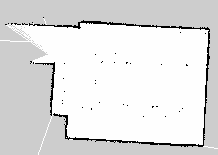
\includegraphics[width=.45\linewidth]{pictures/04/lunch_room/gmapping/angularup100}}} \\
  \subfloat[0 iterations]{\frame{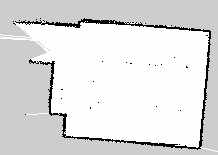
\includegraphics[width=.45\linewidth]{pictures/04/lunch_room/gmapping/iteration00}}} \quad
  \subfloat[10 iterations]{\frame{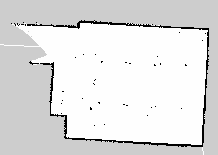
\includegraphics[width=.45\linewidth]{pictures/04/lunch_room/gmapping/iteration10}}} \\
  \subfloat[1 particle]{\frame{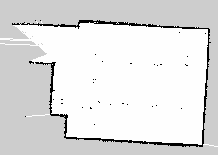
\includegraphics[width=.45\linewidth]{pictures/04/lunch_room/gmapping/particle001}}} \quad
  \subfloat[10 particles]{\frame{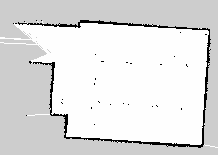
\includegraphics[width=.45\linewidth]{pictures/04/lunch_room/gmapping/particle010}}}
  \caption{Lunch room map varying the linear update rate}
  \label{fig:gmappinglunchres}
\end{figure}  

As it can be sheen on \autoref{fig:gmappinglunchres}, the results are very similar for a wealth of variations in the parameters, therefore it can be concluded that Gmapping has a robust behavior in this scenario. 

\clearpage
\parunder{Hector in\\ Lunch Room} For Hector SLAM, since it can run with or without odometry, tests were run with both cases in mind. \autoref{tab:hectorlunch} summarizes the cases of study (with and without odometry)
\begin{table}[h]
  \centering
  \begin{tabular}{lc}
    \hline
    \textbf{Parameter} & \textbf{Range} \\ \hline
    Default & - \\ \hline
    Multimap resolution & 2 \& 3 \\ \hline
    Linear update rate & {[}0.2-0.6{]} \\ \hline
    Angular update rate & {[}0.4-1.4{]} \\ \hline
  \end{tabular}
  \caption{Tests with Hector in the lunch room}
  \label{tab:hectorlunch}
\end{table}

\autoref{fig:hector3def} shows, the results of the default maps obtained and there is not much difference between them. However, on the left corner of the map there is a small misadjustment that was not seen with Gmapping.
\begin{figure}[h]
  \centering
  \subfloat[With odometry]{\frame{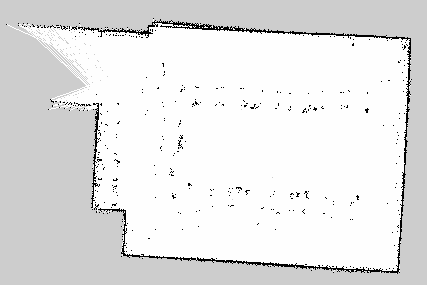
\includegraphics[width=.45\linewidth]{pictures/04/lunch_room/hector/odommulti3default}}} \quad
  \subfloat[Without odometry]{\frame{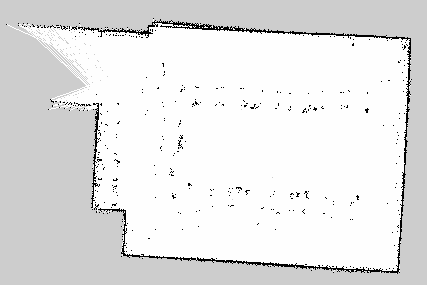
\includegraphics[width=.45\linewidth]{pictures/04/lunch_room/hector/nodommulti3default}}} \\
  \caption{Default results for Hector SLAM (Lunch Room)}
  \label{fig:hector3def}
\end{figure}  

This problem is persistent across all the configurations no matter if using odometry or not (Figures \ref{fig:hector3lin} and \ref{fig:hector3an}). 
\begin{figure}[h]
  \centering
  \subfloat[With odometry]{\frame{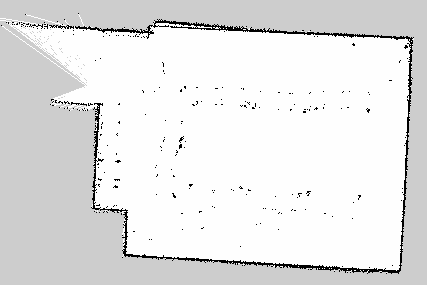
\includegraphics[width=.45\linewidth]{pictures/04/lunch_room/hector/odommulti3linear02}}} \quad
  \subfloat[Without odometry]{\frame{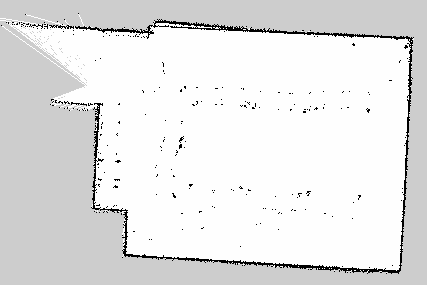
\includegraphics[width=.45\linewidth]{pictures/04/lunch_room/hector/nodommulti3linear02}}} \\
  \caption{Linear update at 0.2 m with Hector (Lunch Room)}
  \label{fig:hector3lin}
\end{figure}  

\begin{figure}[t]
  \centering
  \subfloat[With odometry]{\frame{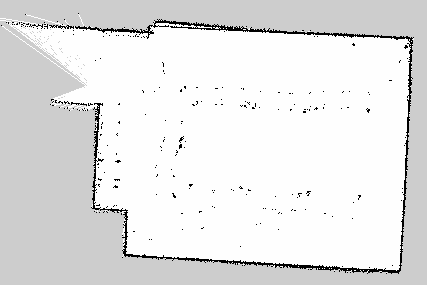
\includegraphics[width=.45\linewidth]{pictures/04/lunch_room/hector/odommulti3linear02}}} \quad
  \subfloat[Without odometry]{\frame{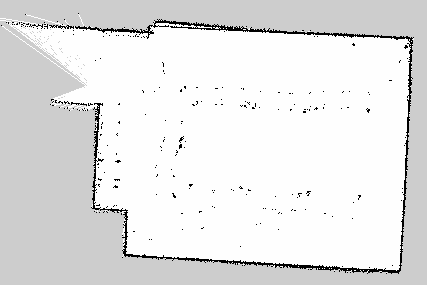
\includegraphics[width=.45\linewidth]{pictures/04/lunch_room/hector/nodommulti3linear02}}} \\
  \caption{Angular update at 0.4 rad with Hector (Lunch Room)}
  \label{fig:hector3an}
\end{figure}  

Thus, it could be due to the map multi resolution parameter, since maps are divided into coarser layers and matches are done with the previous map. In \autoref{fig:hectormulti}, the resolution was changed to 2 and the drift is higher, possibly meaning that the scanmatcher needs more layers. With 4 maps, the drift is barely appreciable, but there is not much change when using 3 layers.

\begin{figure}[h]
  \centering
  \subfloat[Map resolution 2]{\frame{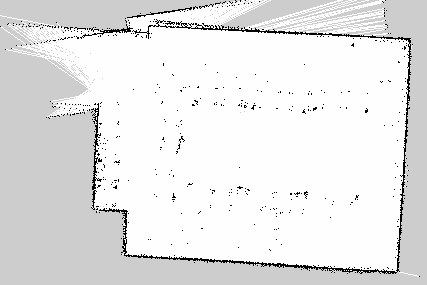
\includegraphics[width=.45\linewidth]{pictures/04/lunch_room/hector/nodommulti2default}}} \quad
  \subfloat[Map resolution 4]{\frame{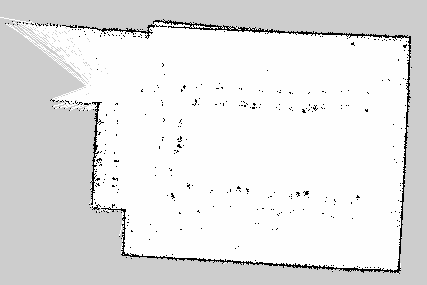
\includegraphics[width=.45\linewidth]{pictures/04/lunch_room/hector/nodommulti4default}}} \\
  \caption{Varying the map resolution with Hector (Lunch Room)}
  \label{fig:hectormulti}
\end{figure}  

Both maps in \autoref{fig:hectormulti} were obtained without odometry, since again there was not any significant change between using or not using it.

The outcome of the mapping process in the lunch room is that Gmapping behaves in a robust fashion and delivers acceptable results without tinkering. On the other hand, with Hector SLAM, results are consistent across configurations but in the overall it lags behind Gmapping.

\subsection{City Science Lab}
The next environment in which the Nexus robot was tested was the City Science (CS) group's laboratory. This room is bigger (around 400m\textsuperscript{2}) and is full of features and obstacles, therefore it is and interesting place to perform SLAM in.

\parunder{Gmapping in CS} The different parameters tested are shown in \autoref{tab:gmappingcs}. The default map is shown in \autoref{fig:gmappingcsdef}. The results are acceptable for most of the area except for the left side of the map, where it is not complete.
\begin{table}[t]
  \centering
  \begin{tabular}{lc}
  \hline
    \textbf{Parameter} & \textbf{Range} \\ \hline
    Default & - \\ \hline
    Linear update rate & {[}0.2-0.6{]} \\ \hline
    Angular update rate & {[}0.4-1.4{]} \\ \hline
    Number of particles in the filter & {[}1-50{]} \\ \hline
    Occupied threshold & {[}0.3-0.9{]} \\ \hline
  \end{tabular}
  \caption{Tests with Gmapping in CS laboratory}
  \label{tab:gmappingcs}
\end{table}

The cause for this to happen would be that region is surrounded by glass doors and acrylic surfaces (grey rectangle embedded on the left part) that compose the base of the CityScope platforms.

\begin{figure}[h]
  \centering
  \frame{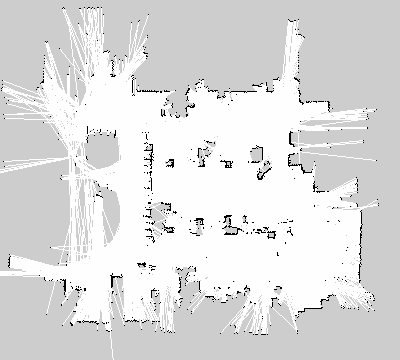
\includegraphics[width=\linewidth]{pictures/04/city_science/gmapping/default}}
  \caption{CS with defaults for Gmapping}
  \label{fig:gmappingcsdef}
\end{figure}  

In order to mitigate this issue, the approaches taken were to vary the linear and angular update rates, as well as the occupied threshold and the particles. Results are shown in \autoref{fig:gmappingcsres}
\begin{figure}[t!]
  \centering
  \subfloat[Linear update at 0.1 m]{\frame{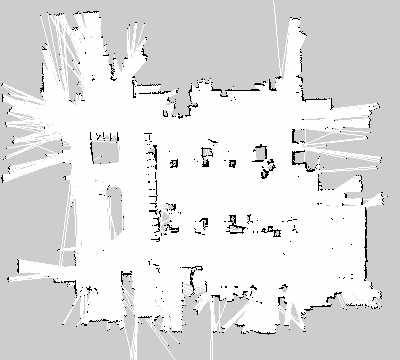
\includegraphics[width=.39\linewidth]{pictures/04/city_science/gmapping/linear010}}} \quad
  \subfloat[Linear update at 0.5 m]{\frame{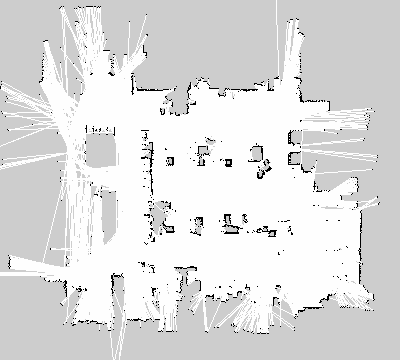
\includegraphics[width=.39\linewidth]{pictures/04/city_science/gmapping/linear050}}} \\
  \subfloat[Angular update at 0.1 rad]{\frame{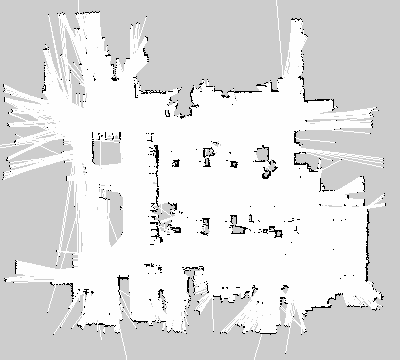
\includegraphics[width=.39\linewidth]{pictures/04/city_science/gmapping/angular010}}} \quad
  \subfloat[Angular update at 1.0 rad]{\frame{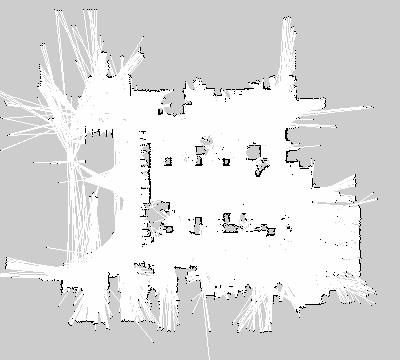
\includegraphics[width=.39\linewidth]{pictures/04/city_science/gmapping/angular100}}} \\
  \subfloat[Occupancy threshold of 0.3]{\frame{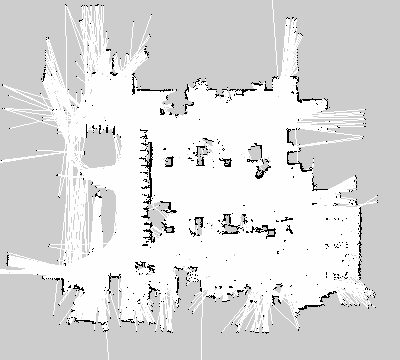
\includegraphics[width=.39\linewidth]{pictures/04/city_science/gmapping/occ03}}} \quad
  \subfloat[Occupancy threshold of 0.8]{\frame{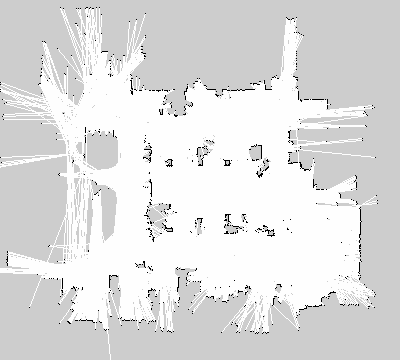
\includegraphics[width=.39\linewidth]{pictures/04/city_science/gmapping/occ08}}} \\
  \subfloat[5 particles]{\frame{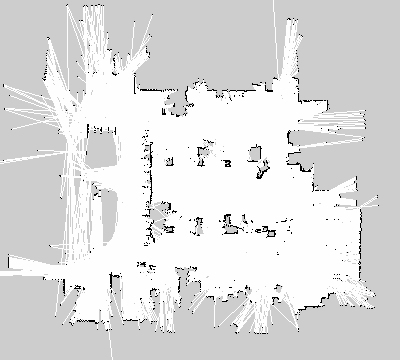
\includegraphics[width=.39\linewidth]{pictures/04/city_science/gmapping/particles05}}} \quad
  \subfloat[50 particles]{\frame{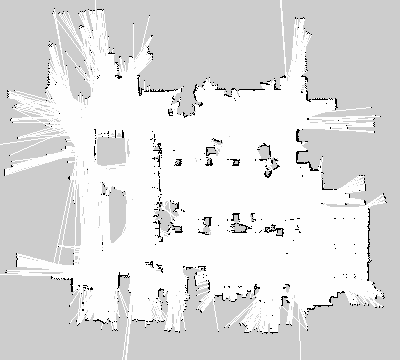
\includegraphics[width=.39\linewidth]{pictures/04/city_science/gmapping/particles50}}}
  \caption{CS results with Gmapping}
  \label{fig:gmappingcsres}
\end{figure}  

From these results, the folowing conclusions can be obtained: increasing the update rate improves the area, but in the case of the linear update there is a limit to the improvement, since with 0.1m, the map starts drifting. For the angular case, this does not occur and a continued lowering of the rate value improves the overall quality.

The reason to vary the occupied threshold in this case was to mitigate the effect of small obstacles or features. In fact, with an occupied threshold of 0.8 there are fewer 'isolated' points but the overall result is 'blurrier'.

With regards to the number of particles, it seems that increasing their number helps mititigate the voids on the left region, due to the fact that with more particles there are more maps and they are able to approximate reality better.

\parunder{Hector in CS} 
The parameters chosen with Hector SLAM are shown in \autoref{tab:hectorcs} (again with and without odometry):
\begin{table}[h]
  \centering
  \begin{tabular}{lc}
  \hline
    \textbf{Parameter} & \textbf{Range} \\ \hline
    Default & - \\ \hline
    Multimap resolution & {[}2-6{]} \\ \hline
    Linear update rate & {[}0.2-0.6{]} \\ \hline
    Angular update rate & {[}0.4-1.4{]} \\ \hline
  \end{tabular}
  \caption{Tests with Hector in CS laboratory}
  \label{tab:hectorcs}
\end{table}

The default maps obtained in both cases show a drift on the lower part that causes the map to be unacceptable (\autoref{fig:hector3defcs}). As Hector SLAM does not perform any background optimization and relies only on the scanmatcher, when the lidar does not detect obstacles (as it happens on the left area) the state becomes drifted.

\begin{figure}[h]
  \centering
  \subfloat[With odometry]{\frame{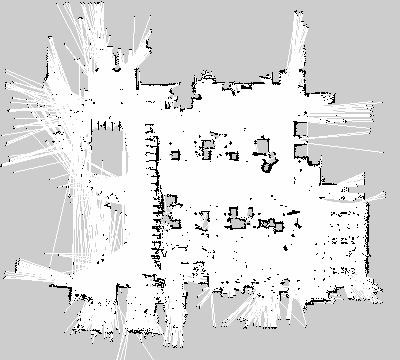
\includegraphics[width=.45\linewidth]{pictures/04/city_science/hector/odommulti3default}}} \quad
  \subfloat[Without odometry]{\frame{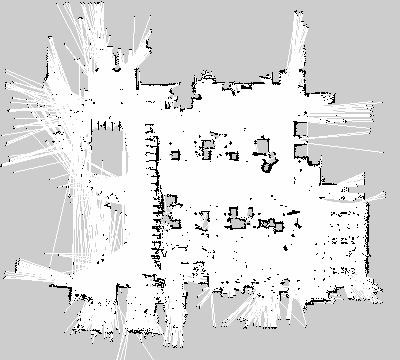
\includegraphics[width=.45\linewidth]{pictures/04/city_science/hector/nodommulti3default}}} \\
  \caption{Default results for Hector SLAM (CS)}
  \label{fig:hector3defcs}
\end{figure}  

To solve this issue 2 approaches were taken: the first one was to increase both linear and angular update rates (Figures \ref{fig:hector3cslin} and \ref{fig:hector3csan}) and the second one to vary the map resolution (\ref{fig:hectorcsmulti}). Again there is no observable difference between using odometry or not meaning that the scanmatcher is barely affected by the errors due to motion estimation.

It can be observed than in the case of the CS laboratory, only the update rates play and important role when tackling the mapping issues. Specially the variation of the linear rate has more visible effects on the improvement of the occupancy grid map.

\begin{figure}[t]
  \centering
  \subfloat[With odometry]{\frame{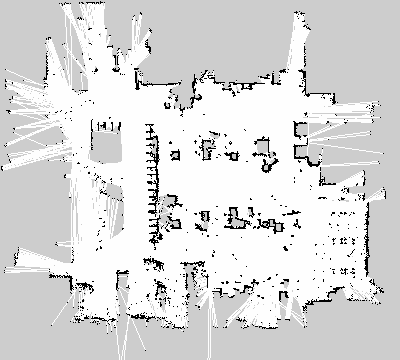
\includegraphics[width=.45\linewidth]{pictures/04/city_science/hector/odommulti3linear020}}} \quad
  \subfloat[Without odometry]{\frame{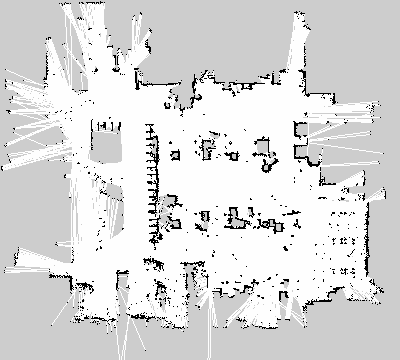
\includegraphics[width=.45\linewidth]{pictures/04/city_science/hector/nodommulti3linear020}}} \\
  \caption{Linear update rate 0.2 m with Hector (CS)}
  \label{fig:hector3cslin}
\end{figure}  

\begin{figure}[t]
  \centering
  \subfloat[With odometry]{\frame{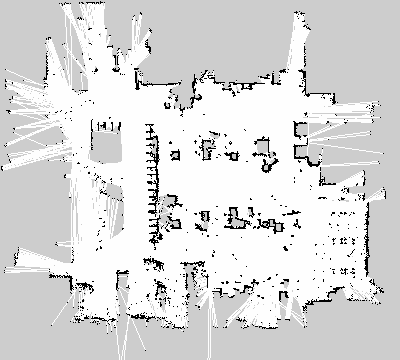
\includegraphics[width=.45\linewidth]{pictures/04/city_science/hector/odommulti3linear020}}} \quad
  \subfloat[Without odometry]{\frame{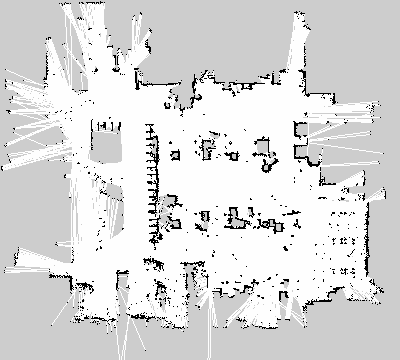
\includegraphics[width=.45\linewidth]{pictures/04/city_science/hector/nodommulti3linear020}}} \\
  \caption{Angular update rate 0.1 rad with Hector (CS)}
  \label{fig:hector3csan}
\end{figure} 

\begin{figure}[t!]
  \centering
  \subfloat[Map resolution 2]{\frame{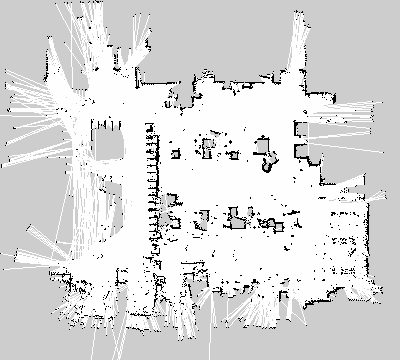
\includegraphics[width=.45\linewidth]{pictures/04/city_science/hector/odommulti2default}}} \quad
  \subfloat[Map resolution 4]{\frame{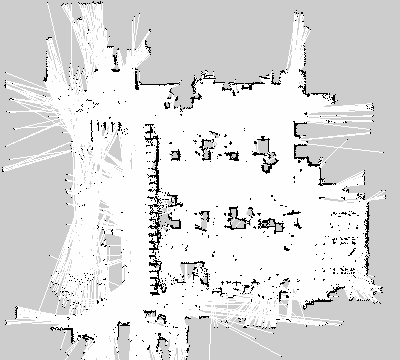
\includegraphics[width=.45\linewidth]{pictures/04/city_science/hector/odommulti4default}}} \\
  \caption{Varying map resolution with Hector (CS)}
  \label{fig:hectorcsmulti}
\end{figure}

This time again results with Gmapping are slightly better. With regards to Hector, for these relatively small scenarios, odometry does not have any effect on the final result of the SLAM.

\subsection{Media Lab 3rd floor}
The last environment tested with the robot was the Media Lab's (ML) third floor. Concerning the area, it is slightly bigger than the City Science laboratory (around 600 m\textsuperscript{2}), but it has both long, featureless corridors and larger open areas. 

\parunder{Gmapping in ML} Since this is a more difficult environment, most of the parameters were varied in order to observe their effect on the environment. everything is summarized on \autoref{tab:gmappingml}.
\begin{table}[h]
  \centering
  \begin{tabular}{lc}
  \hline
    \textbf{Parameter} & \textbf{Range} \\ \hline
    Default & - \\ \hline
    Linear update rate & {[}0.1-1.0{]} \\ \hline
    Angular update rate & {[}0.1-1.0{]} \\ \hline
    Iterations of the scanmatcher & {[}1-10{]} \\ \hline
    Number of particles in the filter & {[}5-50{]} \\ \hline
  \end{tabular}
  \caption{Tests with Gmapping in ML third floor}
  \label{tab:gmappingml}
\end{table}

As with the previous areas, first the default result will be shown (\autoref{fig:gmappingmldef}).
\begin{figure}[h]
  \centering
  \frame{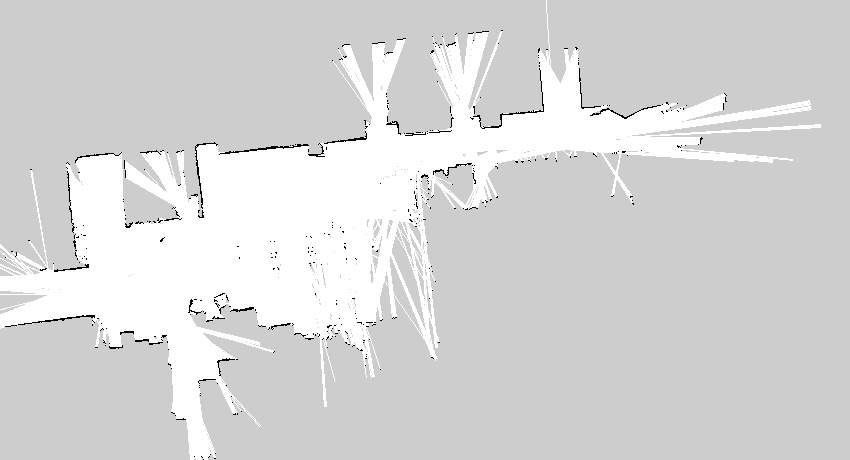
\includegraphics[width=\linewidth]{pictures/04/3rd_floor/gmapping/default}}
  \caption{ML with defaults for Gmapping}
  \label{fig:gmappingmldef}
\end{figure} 

The result in general is acceptable, even though some of the edges are not perfectly matched. As it has been learnt from previous experiences, this effect can be improved by either increasing the linear/angular rates, the iterations of the scanmatcher and the particles in the filter. These results are shown in \autoref{fig:gmappingmlres}. The differences are very subtle, but the best results are obtained by increasing the iterations (\autoref{fig:gmappingmlres}\protect\subref{fig:mlbest}).

\begin{figure}[t!]
  \centering
  \subfloat[Linear update at 0.1 m]{\frame{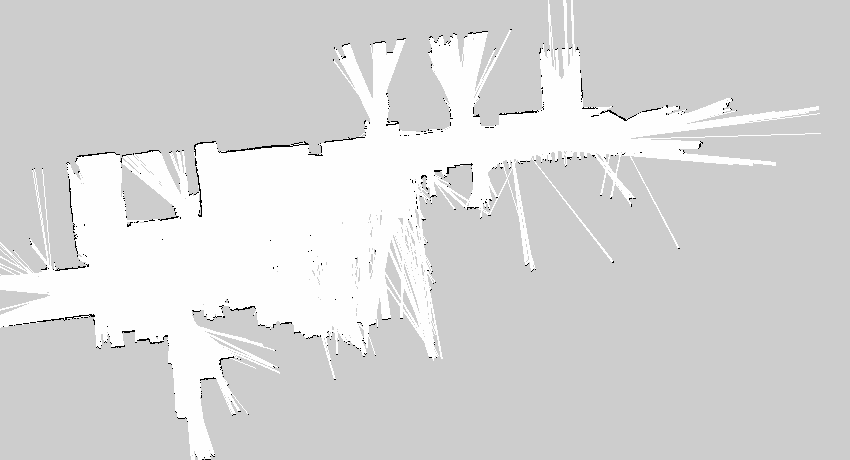
\includegraphics[width=.7\linewidth]{pictures/04/3rd_floor/gmapping/linear010}}} \\
  \subfloat[Angular update at 0.1 m]{\frame{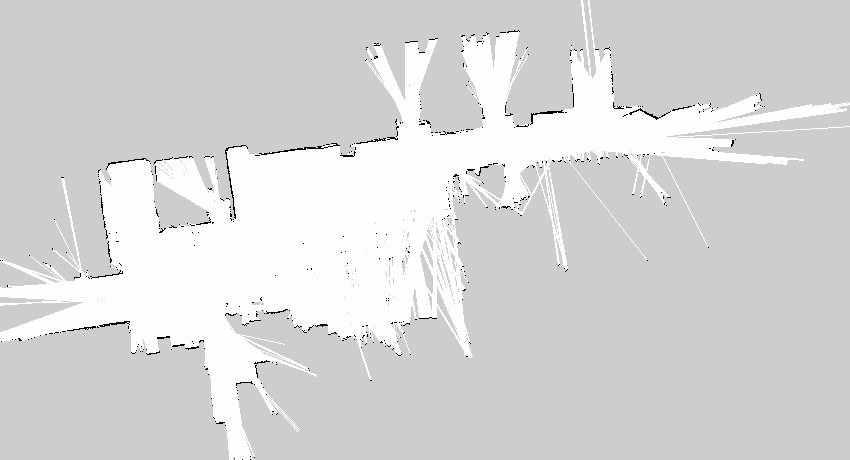
\includegraphics[width=.7\linewidth]{pictures/04/3rd_floor/gmapping/angular010}}} \\
  \subfloat[10 iterations for the scanmatcher]{\frame{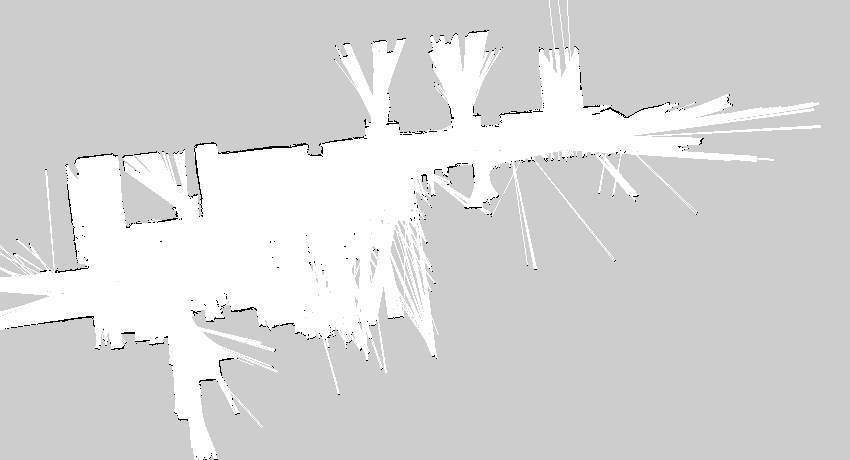
\includegraphics[width=.7\linewidth]{pictures/04/3rd_floor/gmapping/iterations10}} \label{fig:mlbest}} \\
  \subfloat[50 particles on the filter]{\frame{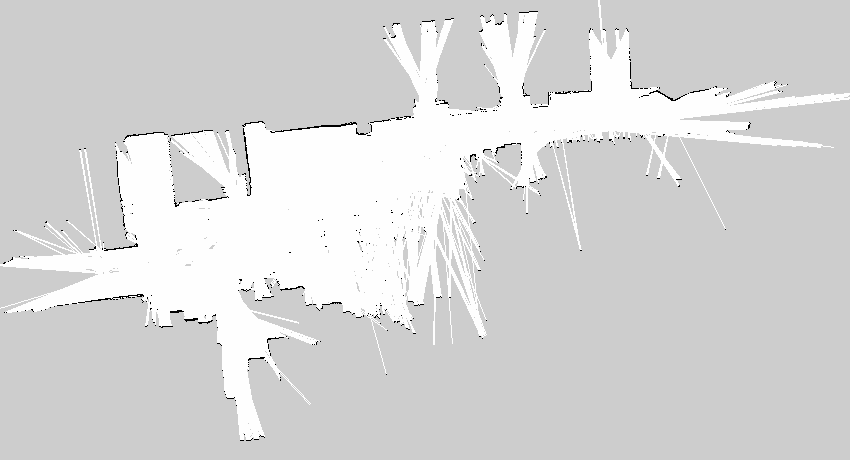
\includegraphics[width=.7\linewidth]{pictures/04/3rd_floor/gmapping/particles50}}} \\
  \caption{Media Lab results with Gmapping}
  \label{fig:gmappingmlres}
\end{figure}

\clearpage
\parunder{Hector in ML} For Hector mapping, parameters are described on \autoref{tab:hectorml}. Results with and without odometry are the same in this case, therefore for the sake of space, results will be given without odometry.
\begin{table}[h]
  \centering
  \begin{tabular}{lc}
  \hline
    \textbf{Parameter} & \textbf{Range} \\ \hline
    Default & - \\ \hline
    Multimap resolution & {[}2-3{]} \\ \hline
    Linear update rate & {[}0.2-0.4{]} \\ \hline
    Angular update rate & {[}0.4-0.9{]} \\ \hline
  \end{tabular}
  \caption{Tests with Hector in ML third floor}
  \label{tab:hectorml}
\end{table}

The default result appears on \autoref{fig:hector3mldef}. In this case it can be noted that the first outcome with Hector SLAM seems slightly better than with Gmapping. Edges are more defined, there is less drift, fewer voids on the central region and the tables and chairs are captured by the mapping process.
\begin{figure}[htb]
  \centering
  \frame{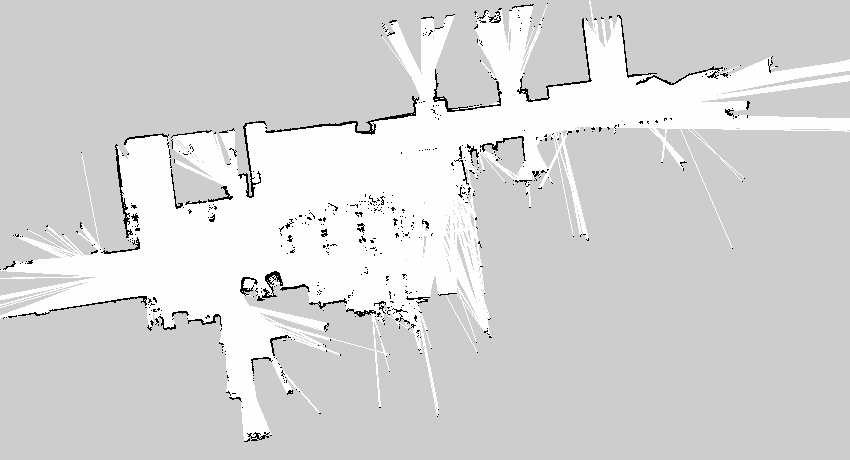
\includegraphics[width=\linewidth]{pictures/04/3rd_floor/hector/nodommulti3default}}
  \caption{Default result for Hector SLAM (ML)}
  \label{fig:hector3mldef}
\end{figure}

The solutions proposed to improve the mapping of the third floor are shown on \autoref{fig:hectormlres} and the strategy is the same as before: increasing the update rate and maintaining map resolution in values of 3 and 2.
\begin{figure}[t!]
  \centering
  \subfloat[Linear update at 0.2 m]{\frame{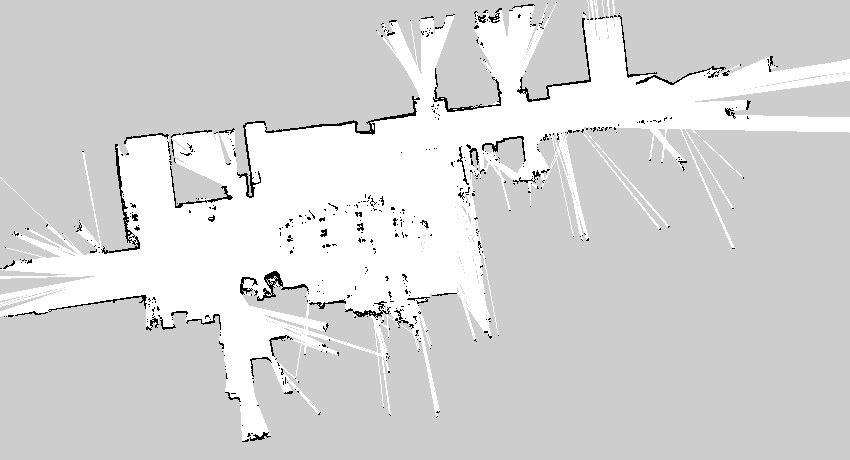
\includegraphics[width=\linewidth]{pictures/04/3rd_floor/hector/nodommulti3linear020}}} \\
  \subfloat[Angular update at 0.4]{\frame{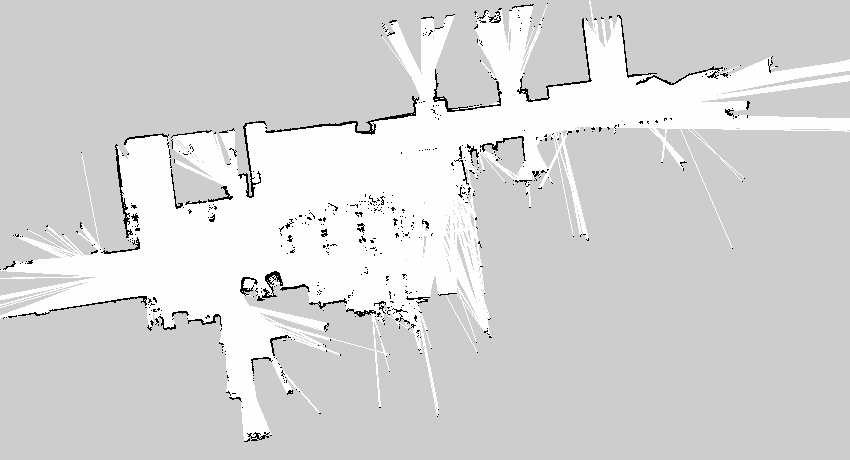
\includegraphics[width=\linewidth]{pictures/04/3rd_floor/hector/nodommulti3angular040}}} \\
  \subfloat[50 particles on the filter]{\frame{\includegraphics[width=\linewidth]{pictures/04/3rd_floor/hector/nodommulti2default}}} \\
  \caption{Results for different configurations in Hector (ML)}
  \label{fig:hectormlres}
\end{figure}

The clearest map is obtained with a linear update of 0.2 m, but the difference is barely noticeable. Features in all maps appear distinct enough and there is no drift on the edges.

The case of the third floor is the first where the results with Hector SLAM are better than with Gmapping. It could be inferred that it could be due to the fact that Gmapping does not scale properly when environments increase in size, but it is still possible to build reasonably good maps in this area.

% \section{Autonomous navigation with Nexus Robot}